% Created by tikzDevice version 0.12.6 on 2026-08-08 12:10:41
% !TEX encoding = UTF-8 Unicode
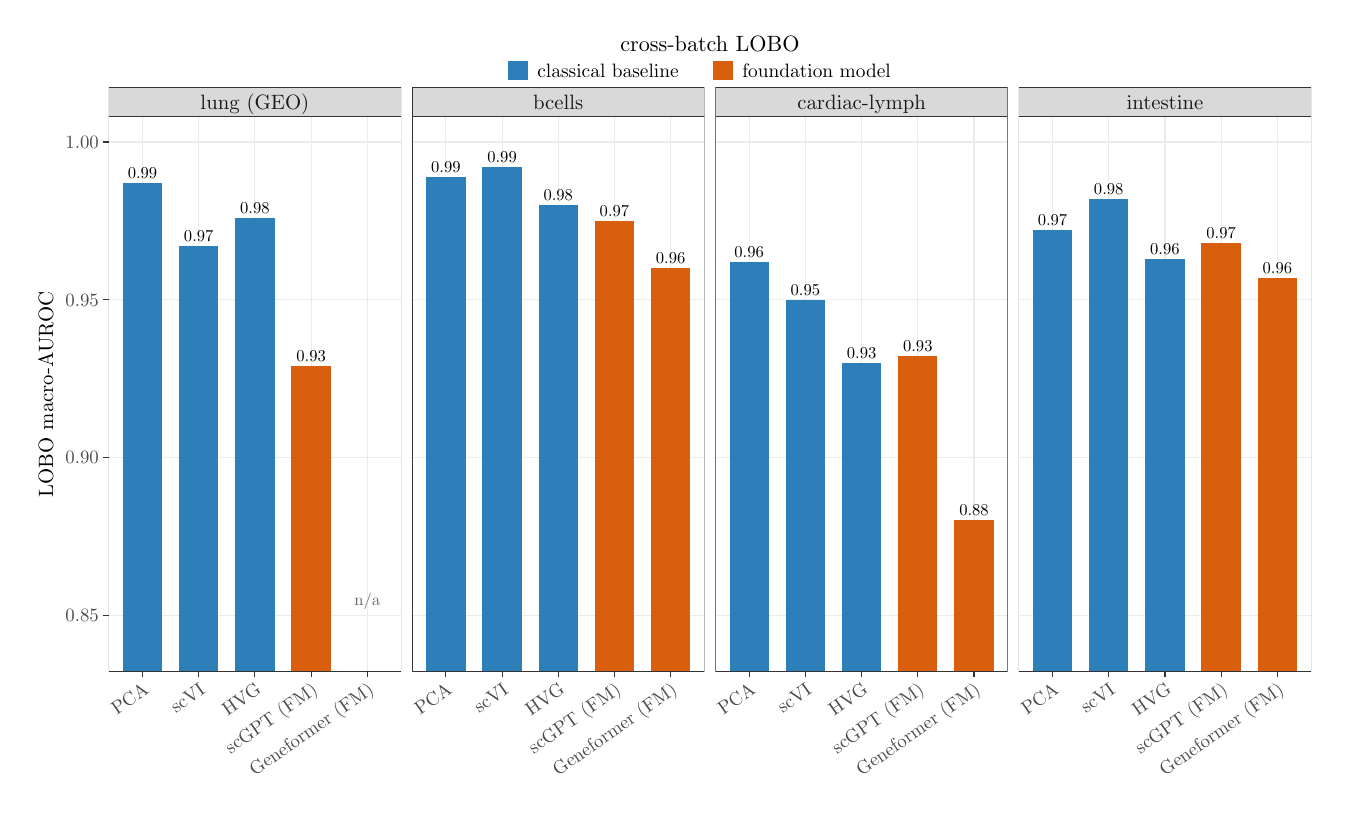
\begin{tikzpicture}[x=1pt,y=1pt]
\definecolor{fillColor}{RGB}{255,255,255}
\path[use as bounding box,fill=fillColor,fill opacity=0.00] (0,0) rectangle (469.75,274.63);
\begin{scope}
\path[clip] (  0.00,  0.00) rectangle (469.75,274.63);
\definecolor{drawColor}{RGB}{255,255,255}
\definecolor{fillColor}{RGB}{255,255,255}

\path[draw=drawColor,line width= 0.4pt,line join=round,line cap=round,fill=fillColor] (  0.00,  0.00) rectangle (469.76,274.63);
\end{scope}
\begin{scope}
\path[clip] ( 29.31, 41.84) rectangle (134.92,242.44);
\definecolor{fillColor}{RGB}{255,255,255}

\path[fill=fillColor] ( 29.31, 41.84) rectangle (134.92,242.44);
\definecolor{drawColor}{gray}{0.92}

\path[draw=drawColor,line width= 0.4pt,line join=round] ( 29.31, 62.36) --
	(134.92, 62.36);

\path[draw=drawColor,line width= 0.4pt,line join=round] ( 29.31,119.34) --
	(134.92,119.34);

\path[draw=drawColor,line width= 0.4pt,line join=round] ( 29.31,176.33) --
	(134.92,176.33);

\path[draw=drawColor,line width= 0.4pt,line join=round] ( 29.31,233.32) --
	(134.92,233.32);

\path[draw=drawColor,line width= 0.4pt,line join=round] ( 41.50, 41.84) --
	( 41.50,242.44);

\path[draw=drawColor,line width= 0.4pt,line join=round] ( 61.81, 41.84) --
	( 61.81,242.44);

\path[draw=drawColor,line width= 0.4pt,line join=round] ( 82.11, 41.84) --
	( 82.11,242.44);

\path[draw=drawColor,line width= 0.4pt,line join=round] (102.42, 41.84) --
	(102.42,242.44);

\path[draw=drawColor,line width= 0.4pt,line join=round] (122.73, 41.84) --
	(122.73,242.44);
\definecolor{fillColor}{RGB}{44,127,184}

\path[fill=fillColor] ( 34.39,-906.43) rectangle ( 48.60,218.50);

\path[fill=fillColor] ( 54.70,-906.43) rectangle ( 68.91,195.71);

\path[fill=fillColor] ( 75.01,-906.43) rectangle ( 89.22,205.97);
\definecolor{fillColor}{RGB}{217,95,14}

\path[fill=fillColor] ( 95.32,-906.43) rectangle (109.53,152.40);
\definecolor{drawColor}{RGB}{0,0,0}

\node[text=drawColor,anchor=base,inner sep=0pt, outer sep=0pt, scale=  0.60] at ( 41.50,220.15) {0.99};

\node[text=drawColor,anchor=base,inner sep=0pt, outer sep=0pt, scale=  0.60] at ( 61.81,197.35) {0.97};

\node[text=drawColor,anchor=base,inner sep=0pt, outer sep=0pt, scale=  0.60] at ( 82.11,207.61) {0.98};

\node[text=drawColor,anchor=base,inner sep=0pt, outer sep=0pt, scale=  0.60] at (102.42,154.04) {0.93};
\definecolor{drawColor}{gray}{0.40}

\node[text=drawColor,anchor=base,inner sep=0pt, outer sep=0pt, scale=  0.60] at (122.73, 66.00) {n/a};
\definecolor{drawColor}{gray}{0.20}

\path[draw=drawColor,line width= 0.4pt,line join=round,line cap=round] ( 29.31, 41.84) rectangle (134.92,242.44);
\end{scope}
\begin{scope}
\path[clip] (138.92, 41.84) rectangle (244.53,242.44);
\definecolor{fillColor}{RGB}{255,255,255}

\path[fill=fillColor] (138.92, 41.84) rectangle (244.53,242.44);
\definecolor{drawColor}{gray}{0.92}

\path[draw=drawColor,line width= 0.4pt,line join=round] (138.92, 62.36) --
	(244.53, 62.36);

\path[draw=drawColor,line width= 0.4pt,line join=round] (138.92,119.34) --
	(244.53,119.34);

\path[draw=drawColor,line width= 0.4pt,line join=round] (138.92,176.33) --
	(244.53,176.33);

\path[draw=drawColor,line width= 0.4pt,line join=round] (138.92,233.32) --
	(244.53,233.32);

\path[draw=drawColor,line width= 0.4pt,line join=round] (151.11, 41.84) --
	(151.11,242.44);

\path[draw=drawColor,line width= 0.4pt,line join=round] (171.42, 41.84) --
	(171.42,242.44);

\path[draw=drawColor,line width= 0.4pt,line join=round] (191.73, 41.84) --
	(191.73,242.44);

\path[draw=drawColor,line width= 0.4pt,line join=round] (212.04, 41.84) --
	(212.04,242.44);

\path[draw=drawColor,line width= 0.4pt,line join=round] (232.35, 41.84) --
	(232.35,242.44);
\definecolor{fillColor}{RGB}{44,127,184}

\path[fill=fillColor] (144.00,-906.43) rectangle (158.22,220.78);

\path[fill=fillColor] (164.31,-906.43) rectangle (178.52,224.20);

\path[fill=fillColor] (184.62,-906.43) rectangle (198.83,210.52);
\definecolor{fillColor}{RGB}{217,95,14}

\path[fill=fillColor] (204.93,-906.43) rectangle (219.14,204.83);

\path[fill=fillColor] (225.24,-906.43) rectangle (239.45,187.73);
\definecolor{drawColor}{RGB}{0,0,0}

\node[text=drawColor,anchor=base,inner sep=0pt, outer sep=0pt, scale=  0.60] at (151.11,222.43) {0.99};

\node[text=drawColor,anchor=base,inner sep=0pt, outer sep=0pt, scale=  0.60] at (171.42,225.85) {0.99};

\node[text=drawColor,anchor=base,inner sep=0pt, outer sep=0pt, scale=  0.60] at (191.73,212.17) {0.98};

\node[text=drawColor,anchor=base,inner sep=0pt, outer sep=0pt, scale=  0.60] at (212.04,206.47) {0.97};

\node[text=drawColor,anchor=base,inner sep=0pt, outer sep=0pt, scale=  0.60] at (232.35,189.38) {0.96};
\definecolor{drawColor}{gray}{0.20}

\path[draw=drawColor,line width= 0.4pt,line join=round,line cap=round] (138.92, 41.84) rectangle (244.53,242.44);
\end{scope}
\begin{scope}
\path[clip] (248.53, 41.84) rectangle (354.14,242.44);
\definecolor{fillColor}{RGB}{255,255,255}

\path[fill=fillColor] (248.53, 41.84) rectangle (354.14,242.44);
\definecolor{drawColor}{gray}{0.92}

\path[draw=drawColor,line width= 0.4pt,line join=round] (248.53, 62.36) --
	(354.14, 62.36);

\path[draw=drawColor,line width= 0.4pt,line join=round] (248.53,119.34) --
	(354.14,119.34);

\path[draw=drawColor,line width= 0.4pt,line join=round] (248.53,176.33) --
	(354.14,176.33);

\path[draw=drawColor,line width= 0.4pt,line join=round] (248.53,233.32) --
	(354.14,233.32);

\path[draw=drawColor,line width= 0.4pt,line join=round] (260.72, 41.84) --
	(260.72,242.44);

\path[draw=drawColor,line width= 0.4pt,line join=round] (281.03, 41.84) --
	(281.03,242.44);

\path[draw=drawColor,line width= 0.4pt,line join=round] (301.34, 41.84) --
	(301.34,242.44);

\path[draw=drawColor,line width= 0.4pt,line join=round] (321.65, 41.84) --
	(321.65,242.44);

\path[draw=drawColor,line width= 0.4pt,line join=round] (341.96, 41.84) --
	(341.96,242.44);
\definecolor{fillColor}{RGB}{44,127,184}

\path[fill=fillColor] (253.61,-906.43) rectangle (267.83,190.01);

\path[fill=fillColor] (273.92,-906.43) rectangle (288.14,176.33);

\path[fill=fillColor] (294.23,-906.43) rectangle (308.45,153.54);
\definecolor{fillColor}{RGB}{217,95,14}

\path[fill=fillColor] (314.54,-906.43) rectangle (328.76,155.82);

\path[fill=fillColor] (334.85,-906.43) rectangle (349.07, 96.55);
\definecolor{drawColor}{RGB}{0,0,0}

\node[text=drawColor,anchor=base,inner sep=0pt, outer sep=0pt, scale=  0.60] at (260.72,191.66) {0.96};

\node[text=drawColor,anchor=base,inner sep=0pt, outer sep=0pt, scale=  0.60] at (281.03,177.98) {0.95};

\node[text=drawColor,anchor=base,inner sep=0pt, outer sep=0pt, scale=  0.60] at (301.34,155.18) {0.93};

\node[text=drawColor,anchor=base,inner sep=0pt, outer sep=0pt, scale=  0.60] at (321.65,157.46) {0.93};

\node[text=drawColor,anchor=base,inner sep=0pt, outer sep=0pt, scale=  0.60] at (341.96, 98.20) {0.88};
\definecolor{drawColor}{gray}{0.20}

\path[draw=drawColor,line width= 0.4pt,line join=round,line cap=round] (248.53, 41.84) rectangle (354.14,242.44);
\end{scope}
\begin{scope}
\path[clip] (358.14, 41.84) rectangle (463.76,242.44);
\definecolor{fillColor}{RGB}{255,255,255}

\path[fill=fillColor] (358.14, 41.84) rectangle (463.75,242.44);
\definecolor{drawColor}{gray}{0.92}

\path[draw=drawColor,line width= 0.4pt,line join=round] (358.14, 62.36) --
	(463.76, 62.36);

\path[draw=drawColor,line width= 0.4pt,line join=round] (358.14,119.34) --
	(463.76,119.34);

\path[draw=drawColor,line width= 0.4pt,line join=round] (358.14,176.33) --
	(463.76,176.33);

\path[draw=drawColor,line width= 0.4pt,line join=round] (358.14,233.32) --
	(463.76,233.32);

\path[draw=drawColor,line width= 0.4pt,line join=round] (370.33, 41.84) --
	(370.33,242.44);

\path[draw=drawColor,line width= 0.4pt,line join=round] (390.64, 41.84) --
	(390.64,242.44);

\path[draw=drawColor,line width= 0.4pt,line join=round] (410.95, 41.84) --
	(410.95,242.44);

\path[draw=drawColor,line width= 0.4pt,line join=round] (431.26, 41.84) --
	(431.26,242.44);

\path[draw=drawColor,line width= 0.4pt,line join=round] (451.57, 41.84) --
	(451.57,242.44);
\definecolor{fillColor}{RGB}{44,127,184}

\path[fill=fillColor] (363.22,-906.43) rectangle (377.44,201.41);

\path[fill=fillColor] (383.53,-906.43) rectangle (397.75,212.80);

\path[fill=fillColor] (403.84,-906.43) rectangle (418.06,191.15);
\definecolor{fillColor}{RGB}{217,95,14}

\path[fill=fillColor] (424.15,-906.43) rectangle (438.37,196.85);

\path[fill=fillColor] (444.46,-906.43) rectangle (458.68,184.31);
\definecolor{drawColor}{RGB}{0,0,0}

\node[text=drawColor,anchor=base,inner sep=0pt, outer sep=0pt, scale=  0.60] at (370.33,203.05) {0.97};

\node[text=drawColor,anchor=base,inner sep=0pt, outer sep=0pt, scale=  0.60] at (390.64,214.45) {0.98};

\node[text=drawColor,anchor=base,inner sep=0pt, outer sep=0pt, scale=  0.60] at (410.95,192.79) {0.96};

\node[text=drawColor,anchor=base,inner sep=0pt, outer sep=0pt, scale=  0.60] at (431.26,198.49) {0.97};

\node[text=drawColor,anchor=base,inner sep=0pt, outer sep=0pt, scale=  0.60] at (451.57,185.96) {0.96};
\definecolor{drawColor}{gray}{0.20}

\path[draw=drawColor,line width= 0.4pt,line join=round,line cap=round] (358.14, 41.84) rectangle (463.75,242.44);
\end{scope}
\begin{scope}
\path[clip] ( 29.31,242.44) rectangle (134.92,253.06);
\definecolor{drawColor}{gray}{0.20}
\definecolor{fillColor}{gray}{0.85}

\path[draw=drawColor,line width= 0.4pt,line join=round,line cap=round,fill=fillColor] ( 29.31,242.44) rectangle (134.92,253.06);
\definecolor{drawColor}{gray}{0.10}

\node[text=drawColor,anchor=base,inner sep=0pt, outer sep=0pt, scale=  0.75] at ( 82.11,245.17) {lung (GEO)};
\end{scope}
\begin{scope}
\path[clip] (138.92,242.44) rectangle (244.53,253.06);
\definecolor{drawColor}{gray}{0.20}
\definecolor{fillColor}{gray}{0.85}

\path[draw=drawColor,line width= 0.4pt,line join=round,line cap=round,fill=fillColor] (138.92,242.44) rectangle (244.53,253.06);
\definecolor{drawColor}{gray}{0.10}

\node[text=drawColor,anchor=base,inner sep=0pt, outer sep=0pt, scale=  0.75] at (191.73,245.17) {bcells};
\end{scope}
\begin{scope}
\path[clip] (248.53,242.44) rectangle (354.14,253.06);
\definecolor{drawColor}{gray}{0.20}
\definecolor{fillColor}{gray}{0.85}

\path[draw=drawColor,line width= 0.4pt,line join=round,line cap=round,fill=fillColor] (248.53,242.44) rectangle (354.14,253.06);
\definecolor{drawColor}{gray}{0.10}

\node[text=drawColor,anchor=base,inner sep=0pt, outer sep=0pt, scale=  0.75] at (301.34,245.17) {cardiac-lymph};
\end{scope}
\begin{scope}
\path[clip] (358.14,242.44) rectangle (463.76,253.06);
\definecolor{drawColor}{gray}{0.20}
\definecolor{fillColor}{gray}{0.85}

\path[draw=drawColor,line width= 0.4pt,line join=round,line cap=round,fill=fillColor] (358.14,242.44) rectangle (463.75,253.06);
\definecolor{drawColor}{gray}{0.10}

\node[text=drawColor,anchor=base,inner sep=0pt, outer sep=0pt, scale=  0.75] at (410.95,245.17) {intestine};
\end{scope}
\begin{scope}
\path[clip] (  0.00,  0.00) rectangle (469.75,274.63);
\definecolor{drawColor}{gray}{0.20}

\path[draw=drawColor,line width= 0.4pt,line join=round] ( 41.50, 39.84) --
	( 41.50, 41.84);

\path[draw=drawColor,line width= 0.4pt,line join=round] ( 61.81, 39.84) --
	( 61.81, 41.84);

\path[draw=drawColor,line width= 0.4pt,line join=round] ( 82.11, 39.84) --
	( 82.11, 41.84);

\path[draw=drawColor,line width= 0.4pt,line join=round] (102.42, 39.84) --
	(102.42, 41.84);

\path[draw=drawColor,line width= 0.4pt,line join=round] (122.73, 39.84) --
	(122.73, 41.84);
\end{scope}
\begin{scope}
\path[clip] (  0.00,  0.00) rectangle (469.75,274.63);
\definecolor{drawColor}{gray}{0.30}

\node[text=drawColor,rotate= 35.00,anchor=base east,inner sep=0pt, outer sep=0pt, scale=  0.68] at ( 44.18, 34.41) {PCA};

\node[text=drawColor,rotate= 35.00,anchor=base east,inner sep=0pt, outer sep=0pt, scale=  0.68] at ( 64.49, 34.41) {scVI};

\node[text=drawColor,rotate= 35.00,anchor=base east,inner sep=0pt, outer sep=0pt, scale=  0.68] at ( 84.80, 34.41) {HVG};

\node[text=drawColor,rotate= 35.00,anchor=base east,inner sep=0pt, outer sep=0pt, scale=  0.68] at (105.11, 34.41) {scGPT (FM)};

\node[text=drawColor,rotate= 35.00,anchor=base east,inner sep=0pt, outer sep=0pt, scale=  0.68] at (125.42, 34.41) {Geneformer (FM)};
\end{scope}
\begin{scope}
\path[clip] (  0.00,  0.00) rectangle (469.75,274.63);
\definecolor{drawColor}{gray}{0.20}

\path[draw=drawColor,line width= 0.4pt,line join=round] (151.11, 39.84) --
	(151.11, 41.84);

\path[draw=drawColor,line width= 0.4pt,line join=round] (171.42, 39.84) --
	(171.42, 41.84);

\path[draw=drawColor,line width= 0.4pt,line join=round] (191.73, 39.84) --
	(191.73, 41.84);

\path[draw=drawColor,line width= 0.4pt,line join=round] (212.04, 39.84) --
	(212.04, 41.84);

\path[draw=drawColor,line width= 0.4pt,line join=round] (232.35, 39.84) --
	(232.35, 41.84);
\end{scope}
\begin{scope}
\path[clip] (  0.00,  0.00) rectangle (469.75,274.63);
\definecolor{drawColor}{gray}{0.30}

\node[text=drawColor,rotate= 35.00,anchor=base east,inner sep=0pt, outer sep=0pt, scale=  0.68] at (153.79, 34.41) {PCA};

\node[text=drawColor,rotate= 35.00,anchor=base east,inner sep=0pt, outer sep=0pt, scale=  0.68] at (174.10, 34.41) {scVI};

\node[text=drawColor,rotate= 35.00,anchor=base east,inner sep=0pt, outer sep=0pt, scale=  0.68] at (194.41, 34.41) {HVG};

\node[text=drawColor,rotate= 35.00,anchor=base east,inner sep=0pt, outer sep=0pt, scale=  0.68] at (214.72, 34.41) {scGPT (FM)};

\node[text=drawColor,rotate= 35.00,anchor=base east,inner sep=0pt, outer sep=0pt, scale=  0.68] at (235.03, 34.41) {Geneformer (FM)};
\end{scope}
\begin{scope}
\path[clip] (  0.00,  0.00) rectangle (469.75,274.63);
\definecolor{drawColor}{gray}{0.20}

\path[draw=drawColor,line width= 0.4pt,line join=round] (260.72, 39.84) --
	(260.72, 41.84);

\path[draw=drawColor,line width= 0.4pt,line join=round] (281.03, 39.84) --
	(281.03, 41.84);

\path[draw=drawColor,line width= 0.4pt,line join=round] (301.34, 39.84) --
	(301.34, 41.84);

\path[draw=drawColor,line width= 0.4pt,line join=round] (321.65, 39.84) --
	(321.65, 41.84);

\path[draw=drawColor,line width= 0.4pt,line join=round] (341.96, 39.84) --
	(341.96, 41.84);
\end{scope}
\begin{scope}
\path[clip] (  0.00,  0.00) rectangle (469.75,274.63);
\definecolor{drawColor}{gray}{0.30}

\node[text=drawColor,rotate= 35.00,anchor=base east,inner sep=0pt, outer sep=0pt, scale=  0.68] at (263.40, 34.41) {PCA};

\node[text=drawColor,rotate= 35.00,anchor=base east,inner sep=0pt, outer sep=0pt, scale=  0.68] at (283.71, 34.41) {scVI};

\node[text=drawColor,rotate= 35.00,anchor=base east,inner sep=0pt, outer sep=0pt, scale=  0.68] at (304.02, 34.41) {HVG};

\node[text=drawColor,rotate= 35.00,anchor=base east,inner sep=0pt, outer sep=0pt, scale=  0.68] at (324.33, 34.41) {scGPT (FM)};

\node[text=drawColor,rotate= 35.00,anchor=base east,inner sep=0pt, outer sep=0pt, scale=  0.68] at (344.64, 34.41) {Geneformer (FM)};
\end{scope}
\begin{scope}
\path[clip] (  0.00,  0.00) rectangle (469.75,274.63);
\definecolor{drawColor}{gray}{0.20}

\path[draw=drawColor,line width= 0.4pt,line join=round] (370.33, 39.84) --
	(370.33, 41.84);

\path[draw=drawColor,line width= 0.4pt,line join=round] (390.64, 39.84) --
	(390.64, 41.84);

\path[draw=drawColor,line width= 0.4pt,line join=round] (410.95, 39.84) --
	(410.95, 41.84);

\path[draw=drawColor,line width= 0.4pt,line join=round] (431.26, 39.84) --
	(431.26, 41.84);

\path[draw=drawColor,line width= 0.4pt,line join=round] (451.57, 39.84) --
	(451.57, 41.84);
\end{scope}
\begin{scope}
\path[clip] (  0.00,  0.00) rectangle (469.75,274.63);
\definecolor{drawColor}{gray}{0.30}

\node[text=drawColor,rotate= 35.00,anchor=base east,inner sep=0pt, outer sep=0pt, scale=  0.68] at (373.02, 34.41) {PCA};

\node[text=drawColor,rotate= 35.00,anchor=base east,inner sep=0pt, outer sep=0pt, scale=  0.68] at (393.33, 34.41) {scVI};

\node[text=drawColor,rotate= 35.00,anchor=base east,inner sep=0pt, outer sep=0pt, scale=  0.68] at (413.64, 34.41) {HVG};

\node[text=drawColor,rotate= 35.00,anchor=base east,inner sep=0pt, outer sep=0pt, scale=  0.68] at (433.95, 34.41) {scGPT (FM)};

\node[text=drawColor,rotate= 35.00,anchor=base east,inner sep=0pt, outer sep=0pt, scale=  0.68] at (454.26, 34.41) {Geneformer (FM)};
\end{scope}
\begin{scope}
\path[clip] (  0.00,  0.00) rectangle (469.75,274.63);
\definecolor{drawColor}{gray}{0.30}

\node[text=drawColor,anchor=base east,inner sep=0pt, outer sep=0pt, scale=  0.68] at ( 25.71, 60.02) {0.85};

\node[text=drawColor,anchor=base east,inner sep=0pt, outer sep=0pt, scale=  0.68] at ( 25.71,117.00) {0.90};

\node[text=drawColor,anchor=base east,inner sep=0pt, outer sep=0pt, scale=  0.68] at ( 25.71,173.99) {0.95};

\node[text=drawColor,anchor=base east,inner sep=0pt, outer sep=0pt, scale=  0.68] at ( 25.71,230.98) {1.00};
\end{scope}
\begin{scope}
\path[clip] (  0.00,  0.00) rectangle (469.75,274.63);
\definecolor{drawColor}{gray}{0.20}

\path[draw=drawColor,line width= 0.4pt,line join=round] ( 27.31, 62.36) --
	( 29.31, 62.36);

\path[draw=drawColor,line width= 0.4pt,line join=round] ( 27.31,119.34) --
	( 29.31,119.34);

\path[draw=drawColor,line width= 0.4pt,line join=round] ( 27.31,176.33) --
	( 29.31,176.33);

\path[draw=drawColor,line width= 0.4pt,line join=round] ( 27.31,233.32) --
	( 29.31,233.32);
\end{scope}
\begin{scope}
\path[clip] (  0.00,  0.00) rectangle (469.75,274.63);
\definecolor{drawColor}{RGB}{0,0,0}

\node[text=drawColor,rotate= 90.00,anchor=base,inner sep=0pt, outer sep=0pt, scale=  0.75] at (  9.17,142.14) {LOBO macro-AUROC};
\end{scope}
\begin{scope}
\path[clip] (  0.00,  0.00) rectangle (469.75,274.63);
\definecolor{fillColor}{RGB}{255,255,255}

\path[fill=fillColor] (172.18,255.06) rectangle (320.88,263.06);
\end{scope}
\begin{scope}
\path[clip] (  0.00,  0.00) rectangle (469.75,274.63);
\definecolor{fillColor}{RGB}{255,255,255}

\path[fill=fillColor] (173.18,255.06) rectangle (181.18,263.06);
\definecolor{fillColor}{RGB}{44,127,184}

\path[fill=fillColor] (173.70,255.58) rectangle (180.66,262.54);
\end{scope}
\begin{scope}
\path[clip] (  0.00,  0.00) rectangle (469.75,274.63);
\definecolor{fillColor}{RGB}{255,255,255}

\path[fill=fillColor] (247.23,255.06) rectangle (255.23,263.06);
\definecolor{fillColor}{RGB}{217,95,14}

\path[fill=fillColor] (247.75,255.58) rectangle (254.71,262.54);
\end{scope}
\begin{scope}
\path[clip] (  0.00,  0.00) rectangle (469.75,274.63);
\definecolor{drawColor}{RGB}{0,0,0}

\node[text=drawColor,anchor=base west,inner sep=0pt, outer sep=0pt, scale=  0.70] at (184.18,256.65) {classical baseline};
\end{scope}
\begin{scope}
\path[clip] (  0.00,  0.00) rectangle (469.75,274.63);
\definecolor{drawColor}{RGB}{0,0,0}

\node[text=drawColor,anchor=base west,inner sep=0pt, outer sep=0pt, scale=  0.70] at (258.23,256.65) {foundation model};
\end{scope}
\begin{scope}
\path[clip] (  0.00,  0.00) rectangle (469.75,274.63);
\definecolor{drawColor}{RGB}{0,0,0}

\node[text=drawColor,anchor=base,inner sep=0pt, outer sep=0pt, scale=  0.80] at (246.53,266.12) {cross-batch LOBO};
\end{scope}
\end{tikzpicture}
